%Every piece of package I've acumulated over the last years
%
%
\documentclass[a4paper,12pt]{article}
\usepackage[utf8]{inputenc}
\usepackage{imakeidx}
\usepackage{graphicx}
\usepackage{float}
\usepackage{amsmath}
\usepackage[backend=bibtex,style=verbose]{biblatex}
\bibliography{bibliography}
\usepackage{csquotes}
\usepackage{tcolorbox}
\usepackage{multirow}
\usepackage{caption}
\usepackage{afterpage}
%End of packages
%
%
%
\begin{document}

\title{Gyroscope}
\author{Gabriel D'Andrade Furlanetto - XDD204950}
\maketitle


\abstract{In this paper, we will analyze the motion of the gyroscope using data collected during University of Salamanca's Mechanics and Waves Laboratory class. We will pay special attention to its rotation and precession, analyze the relation between their frequencies, and then use that data to to calculate the moment of inertia of the principal axis of our system. We will then calculate the moment of inertia by using the gyroscope as a pendulum, and finally compare the two results.}
\pagebreak 
\section{Introduction}

\subsection{Objectives}

The main objective of this paper is to study the gyroscope and its movement, namely its rotation, precession and nutation. Special consideration will be given to the first two, and as such, the frequency of rotation and 

Furthermore, we will calculate the principal moment of inertia of our gyroscope in two different manners: Firstly, using the frequencies of precession and rotation; Then, using a different experimental setup that uses the gyroscope as a pendulum.

\subsection{Theoretical Introduction}
To accurately describe the motion of the gyroscope, a full theory of the rigid solids is necessary. However, anyone who has come in contact with it will know that setting up the Euler Equations and solving them is an extremely non-trivial task that would be way beyond the scope of this section . We will instead consider a simplification where we consider the angular velocity to be large enough\footnote{This approximation is usually referred to as the fast (heavy) symmetrical top, and the general case is called, not surprisingly, the (heavy) symmetrical top. Solutions for the spinning top are usually covered in graduate-level Classical Mechanics texts, with our situation being used as a limiting case. If one wishes to see a detailed solution, \cite[208]{goldstein} is a great resource}. 

\begin{figure}[h!]
\centering
\label{coord_system}
\caption{Coordinate system employed in the solution of the problem}
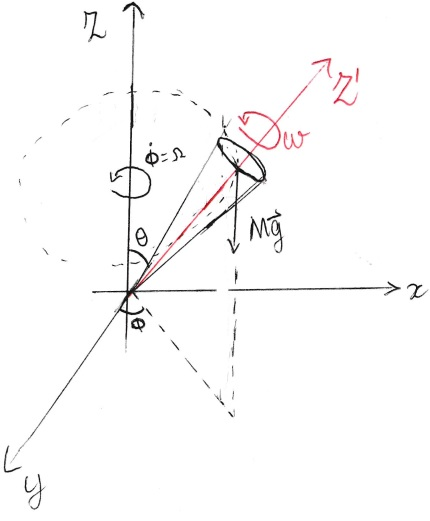
\includegraphics[width=5cm]{coord.jpg}
\end{figure} 

We will start, as is often the case in dynamics, by choosing proper coordinates for our problem. Because of the fact that the distance from the point of contact to the center of mass constant during motion, we will employ spherical polar coordinates $(r,\theta,\phi)$, as represented in Figure \ref{coord_system}. We begin by analyzing the applied torques of the system, of which gravity is the only contributor:

$\boldsymbol{\Gamma} = \boldsymbol{r} \times \boldsymbol{F} = d \boldsymbol{e_r} \times m g \boldsymbol{e_z} = m g d \boldsymbol{e_r} \times (\cos(\theta) \boldsymbol{e_r}-\sin(\theta) \boldsymbol{e_\theta})$

Where d is the distance, M is the mass of the system and g is acceleration due to gravity. If we carry out the trivial calculations, we get that 

\begin{equation}
	\label{torque}
	\boldsymbol{\Gamma} = m g d \sin(\theta) \boldsymbol{e_{\phi}}
\end{equation}

Now, we analyze the system's angular momentum. A priori, there could be a component of angular momentum in each direction, but that would give us a very complicated system to work with in the end. We will instead make use of our approximation and assume that the angular momentum along the axis of rotation, $z'$, dominates the angular momentum as a whole. As such, we write:

\begin{equation}
	\boldsymbol{J} = I \omega \boldsymbol{e_r}
\end{equation}


\section{Experimental Procedure}

\subsection{Measurements}

\section{Results}

\section{Final Discussion}

\end{document}
